\chapter{Edge Offloading \& Early Exiting}

Early exiting model have been used for two purposes in literature.

\begin{enumerate}
	\item Reducing average inference latency and power consumption by letting samples prematurely exit the model based on random distribution \cite{bibid} or predictions able satisfy a confidence threshold criteria exit early exiting \cite{teerapittayanon_branchynet:_2016}.
	\item Comply with application time constraints by exit or sub-model selection. Running only the part of the model possible within the given time frame, reduces wasted computation and a more likely to meet stringent delay constraints  \cite{li_edge_2018}. 
\end{enumerate} 

We propose a more flexible edge offloading scheme, compared to upfront exit selection. We argue, that allowing the edge server to reach as far as possible, within the time budget and continuously sending back increasingly more confident predictions, will in any case achieve at least the same accuracy, as the inference processes of the two schemes are identical. Even though a sub-model exit have been chosen with care, the risk of timeout is still present as both computation and communication delays are not constant. If unexpected delays do occur, it may cause timeouts and lead to lost predictions. However, our scheme reduces the risk of timeouts and lost predictions, as earlier, albeit less accurate predictions, can be used. 

\section{Offloading Scheme}

Figure \ref{fig:offloading-scheme} illustrates the offloading scheme. To not waste idle time on edge server the data is offloaded from the end device, to edge server as soon as acquired. The edge server preprocesses the data, runs the \gls{dnn} inference process, and whenever predictions are obtained it spawns a thread, sending back the result to the end device. The end device then decides the prediction based upon the information received from the edge server.  

\begin{figure}
	\caption[Offloading scheme]{offloading scheme}
	\label{fig:offloading-scheme}
\end{figure} 

\section{Experimental Setup}

\section{Results}

\subsection{Delay Constraint}

How far are we able to in inference process under different time constraints? 

\begin{figure}
	\centering
	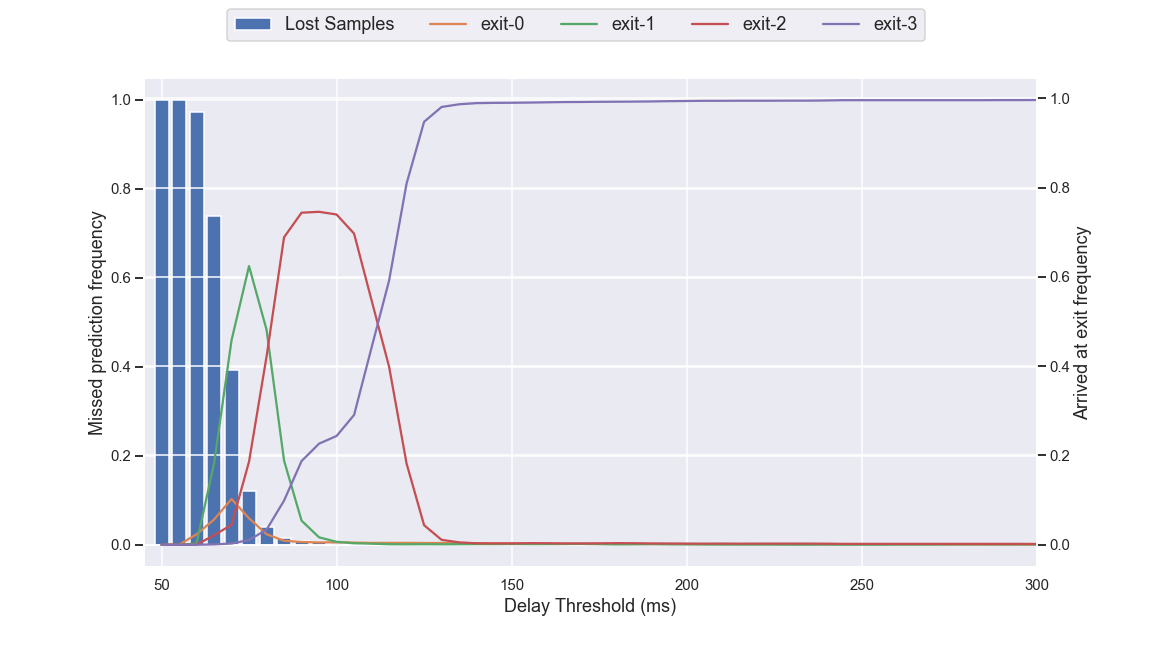
\includegraphics[width=\linewidth]{figures/edge/exit-reached.png}
	\caption[short text]{text}
	\label{fig:exit-reached}
\end{figure}

\subsection{Exit Confidence}

Is $S_{exit_{n}} < S_{exit_{n+1}}$?


\begin{figure}
	\centering
	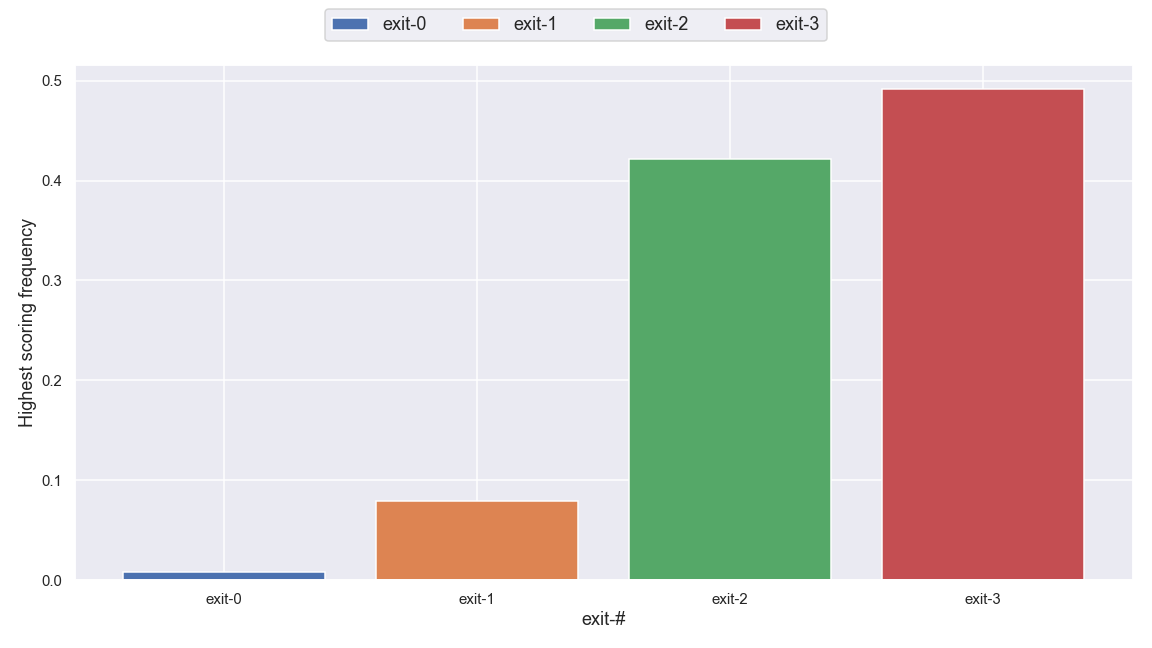
\includegraphics[width=\linewidth]{figures/edge/highest-scoring.png}
	\caption[short text]{text}
	\label{fig:exit-highscore}
\end{figure}

\subsection{Combining Prediction Information}

We define several proposals for using the additional predictions provided from the early exiting framework, with the purpose to improve the accuracy under time constraints. 




We also examined thresholds in the previous chapter, which did show that a high prediction score, have more chance of being correct.       

\begin{description}
	\item[Last Exit] We define the method \emph{last exit}, which is choosing the most confident from the most recent prediction available. In contrast to our finding, that the score is not always better at a later exit, and that the later exit might make a correct prediction from an earlier exit incorrect, the later exit is on average more accurate.
	\item[Confidence (max)] Using all available predictions, we choose the most confident one, i.e. the one with the highest score. Here we neglect the fact, that the later exits are more accurate and assume, that a higher confidence despite the exit leads to a correct prediction.
	\item[Score-margin (max)] We consider all available predictions and determines the score-margin. We select the prediction from the exit with the highest score-margin. From the previous chapter, we know that the score-margin threshold gave a smaller proportion of incorrrectly exited samples at the small cost of samples, that could have been correctly classified using only highest scoring confidence.
	\item[Confidence (add)] We define a method, that additive combines all information from all available predictions and selects the highest scoring class. 
	\item[Score-margin (add)] Similarly we define a method, that determines the score-margin using the two highest scoring classes from each prediction and additive combines the informations.
	\item[Confidence (add,weight)] Almost identical to \emph{confidence (add)}, but uses a weighted sum of all available exits to combine the information. Each exit are weighted to acknowledge the increasing accuracy as the predictions comes from deeper exit in the model.  
	\item[Score-margin (add,weight)] Similarly we define a weighted sum version of the score-margin. 
\end{description}

\begin{figure}
	\centering
	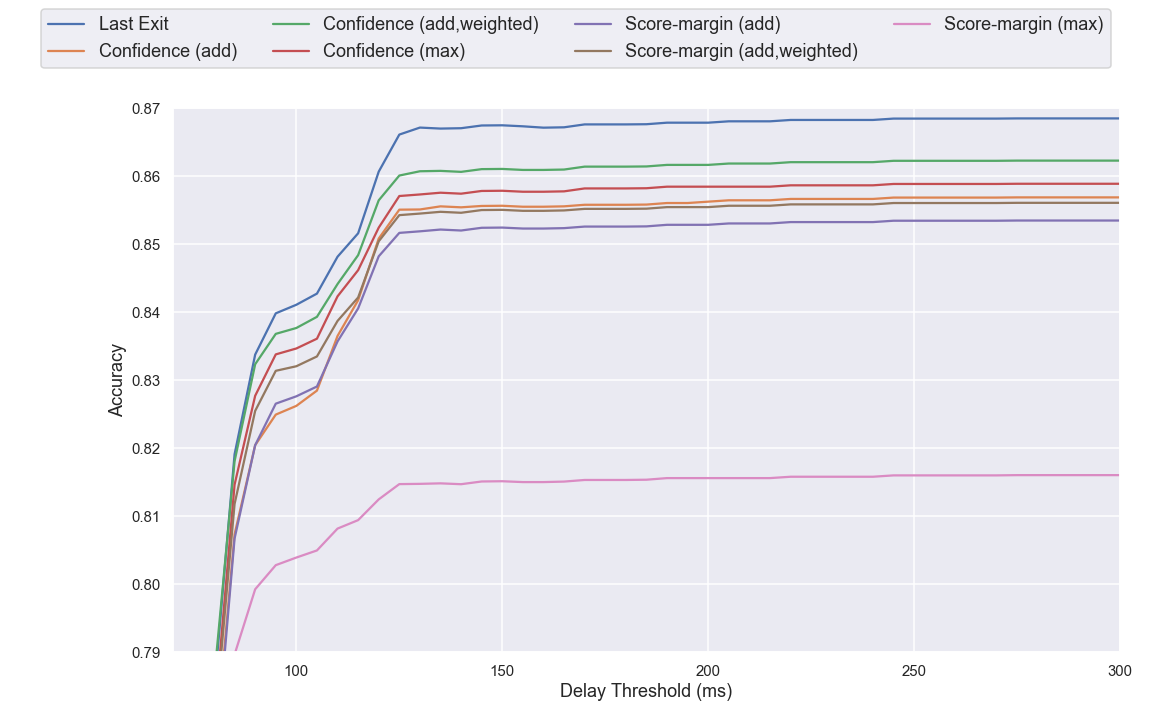
\includegraphics[width=\linewidth]{figures/edge/information-combination.png}
	\caption[short text]{text}
	\label{fig:info-combi}
\end{figure}

Should I create hybrid combinations? Maybe only combine info from exit-0 and -1 and always let exit-2 and -3 have the final say if available? What if we can combine info from those two and omit the poor ones? 